\documentclass[14pt]{article}
\usepackage[a4paper,
            bindingoffset=0.2in,
            left=1.5cm,
            right=1.5cm,
            top=1cm,
            bottom=1cm,
            footskip=.25in]{geometry}
\usepackage{imakeidx}
\usepackage{hyperref}
\hypersetup{hidelinks,
backref=true,
hyperindex=true,
hypertexnames=true,
colorlinks=false,
bookmarks=true,
bookmarksopen=false,
pdftitle={Title},
pdfauthor={Author}}

\usepackage{lipsum}
\usepackage{enumitem}
\usepackage{ifthen}
\usepackage{graphicx}
\usepackage{xcolor}
\hypersetup{
    colorlinks,
    linkcolor={blue!50!black},
    citecolor={blue!50!black},
    urlcolor={blue!80!black}
}
\makeatletter
\newcommand{\mynameis}[1]{%
  \phantomsection#1% Mark hyperlink
  \renewcommand{\@currentlabel}{#1}%
  \renewcommand{\@currentlabelname}{#1}}
\makeatother
\newcounter{probcount}
\newcounter{pcindex}
\newcommand\addProblemPlusSolution[2]{%
  \stepcounter{probcount}
  \expandafter\def\csname P\romannumeral\theprobcount\endcsname{#1}%
  \expandafter\def\csname S\romannumeral\theprobcount\endcsname{#2}%
}
\newcommand\showProblemsThenSolutions{%

      \begin{center}
      \LARGE
        \textbf{Problems}
        \normalsize
\end{center}
  \setcounter{pcindex}{0}%
  \whiledo{\thepcindex < \theprobcount}{%
    \stepcounter{pcindex}%
    \subsection*{\mynameis{Problem \thepcindex}%
                 \label{LP\romannumeral\thepcindex}
                 {\small\mdseries(See \ref{LS\romannumeral\thepcindex})}}

    \csname P\romannumeral\thepcindex\endcsname
  }%

      \newpage
      \begin{center}
      \LARGE
        \textbf{Solutions}
        \normalsize
\end{center}

    \setcounter{pcindex}{0}%
  \whiledo{\thepcindex < \theprobcount}{%
    \stepcounter{pcindex}%
    \subsection*{\mynameis{Solution \thepcindex}%
                 \label{LS\romannumeral\thepcindex}
                 {\small\mdseries(See \ref{LP\romannumeral\thepcindex})}}

    \csname S\romannumeral\thepcindex\endcsname
  }%
}
\makeindex
\begin{document}


% Source
% https://tex.stackexchange.com/questions/175826/avoiding-multiple-label-refs-in-simply-formatted-documents
\begin{titlepage}
    \begin{center}
        \vspace*{1cm}
            
        \Huge
        \textbf{The Great Quiz Book}
            
        \vspace{0.5cm}
        \huge
        Logic \& Math
        
        
\includegraphics[width=8cm]{img/quiz.jpg}
            
        \vspace{1.5cm}
            
        \textbf{Abdullah Al Mahmud}

     \vspace{1.5cm}

	\Large 
	Updated on: \today
	
	
            
        \vfill
            

            
        \vspace{0.8cm}
            

            
        \Large
        www.statmania.info\\
            
    \end{center}
\end{titlepage}

\section{Puzzles}

\addProblemPlusSolution
{
\hrule
\vspace{6pt}
\begin{table}[h]
\centering
\begin{tabular}{|c|c|c|}
\hline
 &  &  \\ \hline
\end{tabular}
\end{table}

There is a combination lock \index{lock} with three digits. The clues are the following:

\begin{table}[h]
\centering
\begin{tabular}{c|c|c}
Digits & \begin{tabular}[c]{@{}c@{}}No. of \\ Correct\\ Digits\end{tabular} & Position \\ \hline
964 & 2 & Wrong \\
286 & 1 & Wrong \\
147 & 1 & Wrong \\
189 & 1 & Correct \\
523 & 0 & NA
\end{tabular}
\end{table}

What is the correct code?
}{

\begin{table}[h]
\centering
\begin{tabular}{|c|c|c|}
\hline
6 & 7 & 9 \\ \hline
\end{tabular}
\end{table}

\textbf{Logic}

\begin{enumerate}[label=(\alph*)]
\item 523 are removed by clue no. 5
\item 1 is removed by clue 3 \& 4 (can't be in right and wrong position simulatenously)
\item 8 is removed by clue 2 \& 4 (can't be in right and wrong position simulatenously)
\item 6 is correct digit by clue 2 (since 2 \& are worng)
\item Position of 6 is 1st (by clue 1 \& 2, both worng position)
\item 9 is the 3rd digit in solution by clue 4 (since 1 \& 8 are incorrect)
\item 4 is removed by clue 1 (since two corret digits are 9 \& 6)
\item The 2nd digit in solution is 7 (by clue 3 and since no other digit exists)
\end{enumerate}


}
\addProblemPlusSolution
{
\hrule
\vspace{6pt}
A shepherd has to cross a river with a sheep, a wolf and a cabbage. Only two can go on the boat, for example, the shepherd and the sheep. How can they cross the river without the wolf eating the sheep and or the sheep eating the cabbage?

}{

\begin{enumerate}
\item Bring sheep
\item Bring back nothing
\item Bring wolf
\item Bring back sheep
\item Bring cabbage
\item Bring back nothing
\item Bring wolf
\end{enumerate}
}

\addProblemPlusSolution
{
\hrule
\vspace{6pt}

A sweet seller receives three opaque boxes. One contains mint sweets, another aniseed sweets, another a mixture of mint and aniseed. The boxes have labels, Mint, Aniseed or Mixture but the seller is told that the labels are all wrongly labeled. What is the minimum number of sweets the man has to take out to verify the contents of the boxes?

}{

There are 6 permutations. If all are labeled wrong, then there are only 2 rotations left.
Opening one box determines the order.

}

\addProblemPlusSolution
{
\hrule
\vspace{6pt}

Inside a hermetically sealed room, there is a light bulb and outside the room there are three switches. Only one of the switches lights the bulb. While the door is closed, one can press the switches as often as you want. But when the door is open, you have to say which of the 3 switches lights the bulb.

}{

Light one. Then turn it off. Then light the second one. Go into the room. If the light is
off and cold, it was the third one.

}


\addProblemPlusSolution
{
\hrule
\vspace{6pt}

How can you time 9 minutes using two sand clocks, with one of 4 minutes and the other of 7 minutes?

}{

Start both sandclocks. Turn the 4 minute clock 4 times, giving 16 minutes. Start counting
after the 7 minutes, when the first sand clock is finished

}


\addProblemPlusSolution
{
\hrule
\vspace{6pt}

A student ask his teacher: how old are your 3 daughters? Teacher: “if you multiply their ages, you get 36. If you add them, you get your house number.” The student protests that it can not be solved. The teacher: “You are right, the oldest plays the piano.” Now the student can answer the question. How old are the daughters?

}{

Look at all the products. We have 6*6*1 = 36*1*1 = 18*2*1 = 6*2*3 = 4*3*3 = 9*2*2 with sums 13,38,21,11,10,13. The sum is ambiguous for 6*6*1 and 9*2*2. The last information gives 9,2,2.

}

\addProblemPlusSolution
{
\hrule
\vspace{6pt}

 \index{door}  \index{guard}  \index{true-false}
 
Imagine two identical doors: behind one is heaven, and behind the other is hell. Each door is guarded by a guardian. One of the guardians always tells the truth, while the other always lies. However, one cannot know which is which. By asking only one question to only one of the two guardians, how can one determine which door leads to heaven?

}{

"What would the other guardian say if I asked them if this is the door to hell?”

}

\addProblemPlusSolution
{
\hrule
\vspace{6pt}

 \index{lock}
\begin{center}
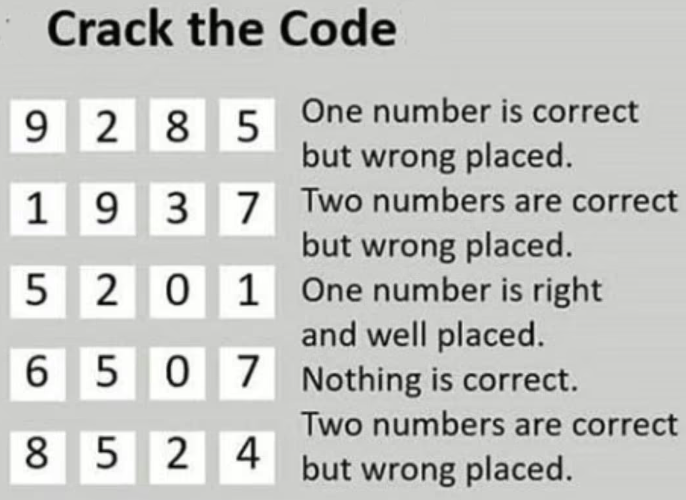
\includegraphics[width=8cm]{img/lock2.png}
\end{center}

}{

\begin{table}[]
\begin{tabular}{|c|c|c|l}
\cline{1-3}
3 & 8 & 4 & 1 \\ \cline{1-3}
\end{tabular}
\end{table}

Explanation

\begin{enumerate}[label=(\alph*)]
\item 0 2 5 6 wwong by 4
\item 1 correct place by 3
\item 4, 8 correct by 5 (since 2, 5 wrong) 
\item 9 wrong by 1 (since only one correct, which is 8)
\item place of 8 is 2nd since it can't take 1st by clue 5, not 3rd by 1st clue, and not 4th by clue 3
\item place of 3 is 1st (since it can't be on 2nd (8), 3rd (wrong) or 4th (1))
\end{enumerate}
}

\addProblemPlusSolution
{
\hrule
\vspace{6pt}

 \index{lock}
\begin{center}
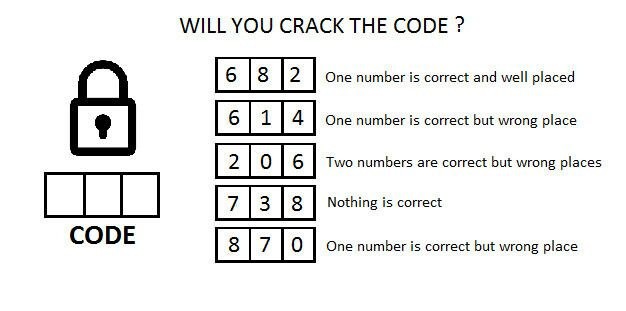
\includegraphics[width=14cm]{img/lock4.jpg}
\end{center}

}{

\begin{table}[h]
\centering
\begin{tabular}{|c|c|c|}
\hline
0 & 4 & 2 \\ \hline
\end{tabular}
\end{table}

Explanation

\begin{enumerate}
\item 0 correct by clue 5 (since 7, 8 wrong)
\item 6 wrong by 1 \& 2 (can't be on wrong and right place simultaneously)
\item 2 in 3rd place by 1 (since 6, 8 wrong), which puts 0 to 1st place (can't be on 2nd or 3rd)
\item We have to find 2nd digit, which is 4 since only other option 1 can't be on 2nd place
\end{enumerate}

}

% PUZZLE END

%START
\addProblemPlusSolution
{
\hrule
\vspace{6pt}

“I only have sheep, goats and horses. In fact, at the moment they are all sheep bar three, all goats bar four and all horses bar five.” How many do I have of each animal?

}{

Three sheep, two goats and one horse

}
%END

%START
\addProblemPlusSolution
{
\hrule
\vspace{6pt}

 I add six to eleven, and get five. Why is this correct?

}{

When it is 11 a.m., adding six hours makes it 5 p.m. 

}
%END

%START
\addProblemPlusSolution
{
\hrule
\vspace{6pt}

Four people (Abid, Basit, Chisti, and Dawud) want to cross a river in a boat that can only carry 100kg. Abid weighs 90kg, Basit weighs 80kg, Chisti weighs 60kg and Dawud weighs 40kg, and they have 20kg of supplies. How do they get across?

}{

\begin{table}[h]
\centering
\begin{tabular}{|c|c|c|c|}
\hline
Go & Return & Stay on Other Side & Stay on this Side \\ \hline
60+40 & 40 & 60 & 20, 40, 80, 90 \\ \hline
90 & 60 & 90 & 20, 40, 60, 80 \\ \hline
60+40 & 40 & 60, 90 & 20, 40, 80 \\ \hline
80+20 & 60 & 20, 80, 90 & 40, 60 \\ \hline
40+60 & - & 20, 40, 60, 80, 90 & - \\ \hline
\end{tabular}
\end{table}

}
%END

%START
\addProblemPlusSolution
{
\hrule
\vspace{6pt}

There are two ducks in front of a duck, two ducks behind a duck and a duck in the middle. How many ducks are there?

}{

Three. Two ducks are in front of the last duck; the first duck has two ducks behind; one duck is between the other two.

}
%END

%START
\addProblemPlusSolution
{
\hrule
\vspace{6pt}

Five people were eating apples, A finished before B, but behind C. D finished before E, but behind B. What was the finishing order?

}{

\begin{center}
CABDE
\end{center}

}
%END

%START
\addProblemPlusSolution
{
\hrule
\vspace{6pt}

Problem

}{

\begin{center}
Solution
\end{center}


}
%END


% MATH START



\section{Mathematics Quizes}

\addProblemPlusSolution
{
\hrule
\vspace{6pt}

The average of 10 numbers is 49. If each of the numbers is divided by 7 and the quotient is then added by 5, what is the changed average number?

}{
\begin{center}
$\frac{49}{7}+5 = 12$
\end{center}
}

%START
\addProblemPlusSolution
{
\hrule
\vspace{6pt}

Let us call all numbers divisible by 11 'Beautiful Numbers'. What is the difference between the largest and smallest five-digit 'Beautiful Number'? 

}{

\begin{center}
Largest: 99990

Smallest: 11110

Difference: 88880
\end{center}

}
%END

%START
\addProblemPlusSolution
{
\hrule
\vspace{6pt}

Using only addition, add eight 8s to get the number 1,000. \index{Math}

}{

888 + 88 + 8 + 8 + 8 = 1,000

}
%END

%START
\addProblemPlusSolution
{
\hrule
\vspace{6pt}

What single digit appears most frequently between and including the numbers 1 and 1,000?

}{

The most common digit is 1! Every number 1–9 appears exactly the same number of times in every ten numbers. But because we included the number 1,000, there’s an extra occurrence of the number 1. In total, the number 1 appears 301 times, and every other number appears 300 times.

}
%END

%START
\addProblemPlusSolution
{
\hrule
\vspace{6pt}

What is the smallest 2-digit number that is equal to seven times the sum of its digits?

}{

10a + b = 7(a + b), then 10a + b = 7a + 7b, and so 3a = 6b, or, more simply, a = 2b. That is, the second digit must be twice the first. The smallest such number is 21.

}
%END

%START
\addProblemPlusSolution
{
\hrule
\vspace{6pt}

What is the smallest number that increases by 12 when it is flipped and turned upside-down?

}{

The answer is 86. When it is turned upside-down and flipped, it becomes 98, which is 12 more than 86.

}
%END

% Put new questions before this line
\showProblemsThenSolutions

\printindex
\end{document}

% Sources

% https://www.rd.com/list/math-riddles/
% BDMO
% Easy short riddles: https://parade.com/947956/parade/riddles/
% Logic puzzle: https://parade.com/970343/parade/logic-puzzles/